\subsection{Algorithmen}
\label{sub:voronoiAlgorithms}
In diesem Kapitel werden die zwei wahrscheinlich meist verwendeten praktische Methoden zur Konstruktion eines Voronoi-Diagramms, das \textit{\textbf{Sweep-}} und das \textit{\textbf{Divide-And-Conquer-Verfahren}}, vorgestellt und hinsichtlich deren Laufzeitverhalten, Komplexität sowie deren Vor- und Nachteile untersucht.

Dabei wird nur der einfachste Fall untersucht: Die Konstruktion eines Voronoi-Diagramm aus einer Menge $S$ mit $n$ Punkten auf der euklidischen Ebene $\mathbb{R}^2$. Das Voronoi-Diagramm $V(S)$ soll dabei möglichst effizient berechnet werden.

Da ein Voronoi-Diagramm $V(S)$ und die Delaunay-Triangulation $DT(S)$ dual zueinander sind, genügt es eine der beiden Struktur zu berechnen. Die andere Struktur lässt
sich in der Zeit \glslink{bigOh}{$O(n)$} daraus ableiten~\parencite[S. 232]{klein2005algorithmischegeometrie}.

Als Grundlage zur Messung der Distanz kommt die \glslink{euclideanDistance}{euklidische Metrik} zum Einsatz. Der Einfachheit halber wird angenommen, dass keine drei Punkte aus $S$ auf einer gemeinsamen Geraden liegen, was bedeutet, dass das Voronoi-Diagramm $V(S)$ zusammenhängend ist und nur Voronoi-Knoten vom Grad drei enthält. Dies hat zur Folge, dass die Delaunay-Triangulation von S $DT(S)$ effektiv eine Triangulation von $S$ ist.

Alle nachfolgend vorgestellten Algorithmen sind optimal, insofern sie das Voronoi-Diagramm $V(S)$ in der Zeit $O(n \log(n))$ und mit Speicherplatz $O(n)$ berechnen~\parencite[S. 269]{klein2005algorithmischegeometrie}.

\newpage{}

\subsubsection{Sweep-Verfahren}
\label{ssub:voronoiAlgorithmsSweep}
Grundsätzlich funktioniert das Sweep-Verfahren so, dass man eine bestimmte Eigenschaft einer Menge von Objekten ermitteln möchte. Dazu werden alle Objekte der Reihe nach besucht und für alle bereits besuchten Objekte werden geeignete Informationen (welche je nach Anwendungsfall variieren) abgelegt. Aus den Informationen ergibt sich schlussendlich die gesuchte Eigenschaft.

Um den Sweep-Algorithmus auf ein Voronoi-Diagramm anwenden zu können, werden beim Sweepen nur die Teile des Voronoi-Diagramms gespeichert, welche links der Sweep-Line $L$ liegen und sich nicht mehr ändern können. Dies heisst, dass kein Punkt rechts von $L$ das Gebiet links der Sweep-Line beeinflusst. Konkret werden die $n$ Punkte aus $S$ in der Reihenfolge aufsteigender X-Koordinaten sortiert und dann jeweils der \gls{bisector} zwischen einem Punkt aus $S$ und der Sweep-Line $L$ in Form einer Parabel $B(p_j, L)$ gebildet. Dies ergibt schlussendlich den Rand der Voronoi-Region, bestehend aus Parabelbögen, genannt \textit{\textbf{Wellenfront}} $W$. Die Parabeln folgen dabei der Sweep-Line mit halber Geschwindigkeit~\parencite[S. 288]{klein2005algorithmischegeometrie}.

Der Schnittpunkt zweier benachbarter Stücke der Wellenfront $W$, z.B. $B(r, L) \cap B(s, L)$, rückt mit fortschreitender Sweep-Line längs deren geraden Bisektors $B(r, s)$ vor. ``Die Verlängerung dieser Bisektoren nach rechts über die Wellenfront hinaus werden \textbf{\textit{Spikes}} genannt'' definiert~\citeauthor{klein2005algorithmischegeometrie} (\citeyear[S. 289]{klein2005algorithmischegeometrie}).

Mit Fortschreiten der Sweep-Line ist es natürlich möglich, dass ein Wellenstück verschwindet, da es den Schnittpunkt seiner beiden Spikes erreicht, und, dass ein neues Wellenstück erscheint, wenn die Sweep-Line $L$ auf einen neuen Punkt $p$ aus $S$ trifft.

Um schlussendlich das Voronoi-Diagramm $V(S)$ von $S$ zu bilden, wird $V(S)$ von Ereignis zu Ereignis erweitert. Wenn kein Ereignis mehr zu bearbeiten ist, wird die Sweep-Line entfernt und alle noch vorhandenen Spikes werden als unbeschränkte Voronoi-Kanten zu $V(S)$ hinzugefügt~\parencite[S. 289 bis 291]{klein2005algorithmischegeometrie}.

Wird eine möglichst effiziente Datenstruktur zur Speicherung des Voronoi-Diagramms $V(S)$, wie etwa die Sweep-Status-Struktur und die Ereignis-Struktur wie von~\citeauthor{klein2005algorithmischegeometrie} vorgeschlagen, bleibt die Grösse in $O(n)$ und die Laufzeit $O(n \log(n))$ (\citeyear[S. 294]{klein2005algorithmischegeometrie}).

\newpage{}

Folgende Darstellungen\footnote{Eigene Darstellung mittels Geogebra} zeigen das Fortschreiten der Sweepline und die Entsteheung einer Voronoi-Kante:

\begin{minipage}[t]{0.5\textwidth}
    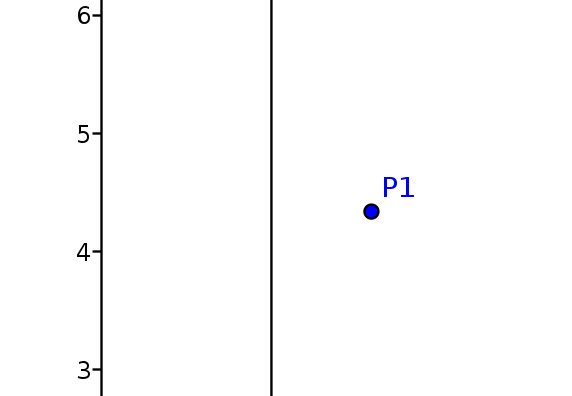
\includegraphics[width=\textwidth]{images/sweep_line_01.png}
    \captionof{figure}{Sweepline ``vor'' Punkt $P1$}
\label{fig:delaunayExample01Orig}
\end{minipage}
\begin{minipage}[t]{0.5\textwidth}
    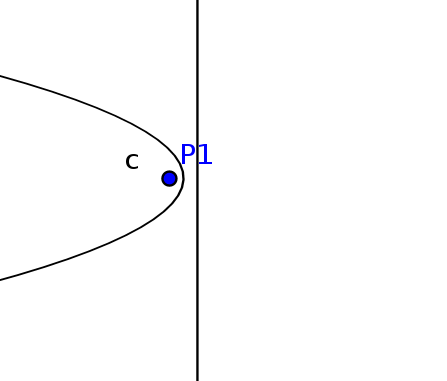
\includegraphics[width=\textwidth]{images/sweep_line_02.png}
    \captionof{figure}{Sweepline ``nach'' $P1$ mit Bisektor $B(P1, L)$}
\label{fig:delaunayExample01500}
\end{minipage}

\begin{minipage}[t]{0.5\textwidth}
    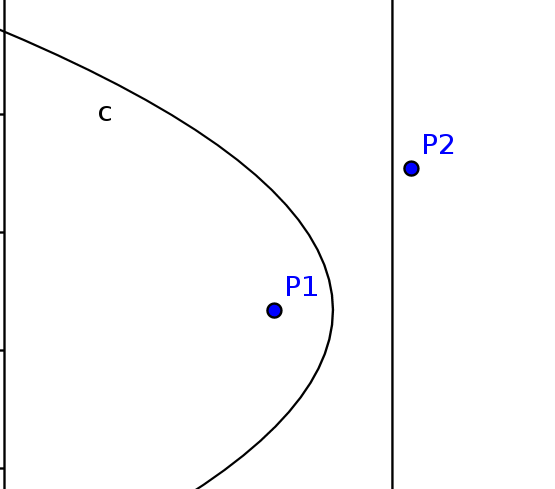
\includegraphics[width=\textwidth]{images/sweep_line_03.png}
    \captionof{figure}{Sweepline ``nach'' $P1$, ``vor'' $P2$}
\label{fig:delaunayExample018000}
\end{minipage}
\begin{minipage}[t]{0.5\textwidth}
    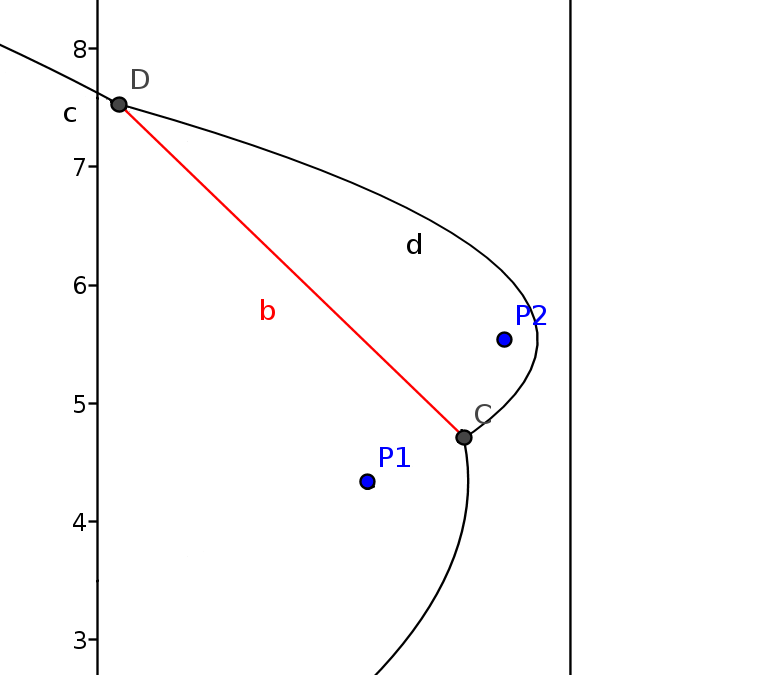
\includegraphics[width=\textwidth]{images/sweep_line_04.png}
    \captionof{figure}{Sweepline ``nach'' $P1$ und $P2$ mit Voronoi-Kante $b$}
\label{fig:delaunayExample018000}
\end{minipage}

\newpage{}
\subsubsection{Divide-and-Conquer-Verfahren}
\label{ssub:voronoiAlgorithmsDivAndConq}
Gemäss~\citeauthor{goodrich2002algorithm} besteht das Divide-and-Conquer-Verfahren (zu Deutsch ``Teile und Herrsche'') grundsätzlich aus drei Schritten:

\begin{compactitem}
\item \textbf{Divide (Teilen)}: Ist ein (Teil-) Problem kleiner als ein gewisser Schwellwert (z.B. ein oder zwei Elemente), wird das (Teil-) Problem mit einer direkten Methode gelöst und danach das Resultat zurückgegeben. Andernfalls wird das (Teil-) Problem in zwei oder mehrere, möglichst gleichgrosse Teilprobleme aufgeteilt (\citeyear{goodrich2002algorithm}, S. 210).

    \item \textbf{Recur (Wiederholen)}: Die Teilprobleme werden rekursiv gelöst.

    \item \textbf{Conquer (Erobern)}: Die Lösungen der Teilprobleme werden zu einer Gesamtlösung des ursprünglichen Problems zusammengefügt (ebd.).

\end{compactitem}

Nach~\citeauthor{shamos1975closestpoint} kann das Divide-and-Conquer-Verfahren zur Erzeugung eines Voronoi-Diagramms $V(S)$ eingesetzt werden. Ein zentraler Aspekt ist hierbei, die $n$-elementige Menge $S$ mittels sogenannten \textit{\textbf{Splitgeraden}}, welche horizontal oder vertikal sind, in Teilmengen zu zerteilen (S. 151 bis 162).

Laut~\citeauthor{klein2005algorithmischegeometrie} führt dies zu folgendem Initialisierungsaufwand für den \textbf{Divide-Schritt}: ``Nach $O(n \log{n})$ Vorbereitungszeit lässt sich die Punktemenge $S$ rekursiv durch achsenparallele Splitgeraden so zerlegen, dass jeder Zerlegungsschritt einer Teilmenge $T$ in Zeit $O(|T|)$ ausgeführt werden kann und zwei Teilmengen mit Mindestgrösse $1/4(|T| - 1)$ liefert'' (\citeyear{klein2005algorithmischegeometrie}, S. 295).

Ein weiterer zentraler Aspekt ist nun die Frage, wie schnell sich zwei Voronoi-Diagramme, z.B. $V(R)$ und $V(S)$ zu einem gemeinsamen Voronoi-Diagramm, also $V(R \in S)$, zusammensetzen (\textbf{Conquer-Schritt}) lassen. Hierzu müssen zwei Arten von Voronoi-Kanten unterschieden werden: Kanten, deren Punkte zu derselben Teilmenge $R$ oder $S$ gehören und Kanten, die zwischen den beiden Regionen verlaufen. Diese Kanten bilden den Bisektor der beiden Teilmengen $B(R,S)$, oder, laut dem Autor~\citeauthor{klein2005algorithmischegeometrie}: ``$V(R)$ und $V(S)$ werden mit dem Faden $B(R,S)$ zusammengenäht, und die überstehenden Stücke werden abgeschnitten''. Die schwierigste Aufgabe ist also die Konstruktion des Bisektors. Alle anderen Schritte können dann in der Zeit $O(n)$ vorgenommen werden~\parencite[S. 297 bis 298]{klein2005algorithmischegeometrie}.

\newpage{}

\begin{figure}[h]
\centering
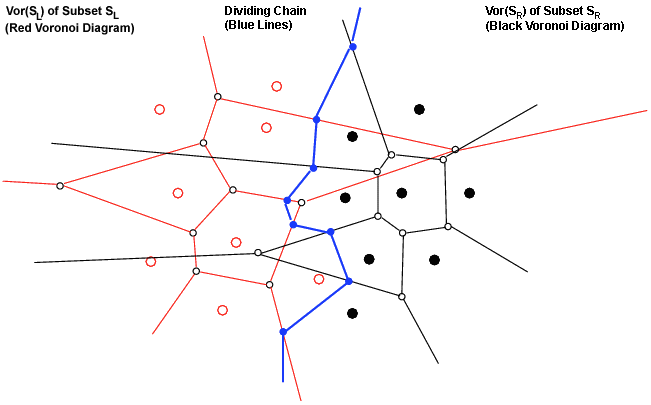
\includegraphics[width=200px]{images/voronoi_divide_conquer_01.png}
\caption{Beispiel des Bisektors $B(R,S)$\protect\footnotemark, blau dargestellt}
\label{fig:voronoiRegionExample01}
\end{figure}
\footnotetext{\cite{rmuhamma2010}}

Das Erstellen des Bisektors der beiden Voronoi-Regionen geschieht in zwei Phasen. Zuerst wird eines der unbeschränkten Endstücke von $B(R,S)$ gesucht, dann verfolgt man den Bisektor durch beide Voronoi-Diagramme $V(R)$ und $V(S)$ bis man bei dem anderen Endstück von $B(R,S)$ angelangt ist.

Um eines der unbeschränkten Endstücke von $B(R,S)$ zu finden, werden die beiden Regionen $V(R)$ und $V(S)$ quasi übereinandergelegt. Dabei kann der Durchschnitt zweier unbeschränkter Regionen $VR(p, R) \cap VR(q, S)$ leer, beschränkt oder aber unbeschränkt sein. Die unbeschränkten Durchschnitte werden der Reihe nach besucht und es wird getestet ob ein unbeschränktes Stück von $B(R,S)$ darin vorkommt. Ist dies der Fall, so wurde ein Endstück von $B(R,S)$ gefunden. Daraus folgt, wie \citeauthor{klein2005algorithmischegeometrie} sagt: ``Sind $V(L)$ (hier $V(R)$) und $V(R)$ (hier $V(S)$) vorhanden, so lässt sich ein Endstück von $B(L,R)$ (hier $B(R,S)$) in Zeit $O(n)$ finden''~\parencite[S. 298 bis 299]{klein2005algorithmischegeometrie}.

Bei der zweiten Phase geht es nun um die Weiterverfolgung des Bisektors $B(R,S)$ durch die beiden Diagramme $V(R)$ und $V(S)$. Grundsätzlich wird nun eine konvexe Hülle der beiden Diagramme erzeugt, danach wird folgendes Schema angewendet bis der Bisektor, bzw.\ das andere unbeschränkte Endstück, erreicht ist:

\begin{compactitem}
  \item Bisektor $B(r,s)$ der gerade betrachteten Punkte finden
  \item Für den Bisektor wird nun Folgendes bestimmt:
  \begin{compactitem}
    \item der Schnittpunkt $r$ mit der Region $V(R)$, an welchem der Bisektor im letzten Schritt nicht abgeschnitten wurde
    \item der Schnittpunkt $s$ mit der Region $V(S)$, an welchem der Bisektor im letzten Schritt nicht abgeschnitten wurde
    \item die Nachbaren $r'$ und $s'$, welche mit den Schnittpunkten $R$ und $S$ des Bivekorts die Kante gemeinsam haben, auf welcher $r$ und $s$ liegen
  \end{compactitem}
\end{compactitem}

Ist nun der Schnittpunkt $s$ höher als $r$, wird $V(S)$ durch $s'$ ersetzt und der aktuelle betrachtete Bisektor $B(r,s)$ an dem Schnittpunkt $s$ abgeschnitten.
Ist aber der Schnittpunkt $r$ höher als $s$, wird $V(R)$ durch $r'$ ersetzt und der aktuelle betrachtete Bisektor $B(r,s)$ an dem Schnittpunkt $r$ abgeschnitten.
Danach wird der neue aktuelle Bisektor $B(r,s)$ gemäss obigem Schema bestimmt.

Es ist möglich, dass der Bisektor eine Region mehrfach besucht und dabei dasselbe Stück des Randes mehrfach durchläuft, was zu einer höheren Komplexität führt. Es genügt jedoch die linken unbeschränkten Regionen \textit{im Uhrzeigersinn} und die rechten unbeschränkten Regionen \textit{gegen den Uhrzeigersinn} zu durchlaufen und sich dabei den zuletzt gefundenen und verworfenen Schnittpunkt als Abbruchbedingung zu merken (Details siehe~\cite[S. 301]{klein2005algorithmischegeometrie}).

Somit lässt sich ein Voronoi-Diagramm aus $n$-Punkten in einer Ebene in der Zeit $O(n \log{n})$ und linearem Speicherplatz konstruieren~\parencite[S. 299 bis 302]{klein2005algorithmischegeometrie}.

\subsection{Vergleich}
\label{ssec:voronoiAlgorithmsComparison}

Betrachtet man die beiden Verfahren im Vergleich, so stellt man fest, dass deren Laufzeit, wie auch deren Speicherplatzbedarf derselbe ist, nämlich $O(n \log{n})$ bzw. $O(n)$.

Der einzige offensichtliche Vorteil des Divide-and-Conquer-Verfahrens könnte sich in der möglichen Parallelität zeigen. Die einzelnen Teilprobleme könnten heutzutage problemlos parallel auf mehreren Kernen gelöst werden. Allerdings bringt dies sicherlich wiederum etwas Aufwand zur Synchronisierung mit sich. Beim Sweep-Verfahren wäre dies wohl nicht möglich, da dort gilt, dass alles, was sich links, der Sweep-Line befindet nicht mehr von Änderungen beeinflusst werden darf.

